\chapter{State of the Art}
\label{chapter:state_of_the_art}

This chapter starts by covering background concepts about anticipation in biology, \acl{ml} and collaborative robotics and then reviews previous work related to the dissertation theme, including sensors and methods.

\section{Background Material}

\subsection{Anticipation in Biology}

Anticipation is a research topic in many areas, such as biology, brain studies, psychology, social sciences, artificial intelligence, and engineering. One of the most cited definitions in the last decades and across the various fields is Rosen's \cite{Rosen1985}:

\begin{displayquote}
An anticipatory system is a system containing a predictive model of itself and/or its environment, which allows it to change state at an instant in accord with the model's predictions pertaining to a later instant.
\end{displayquote}

In the field of biology, \textcite{Louie2010} claims that \textquote{Much, if not most, biological behavior is model-based ...} with the referred models being the \textquote{... internal predictive models of themselves and their environments ...}. \textcite{Poli2010} further claims that \textquote{... given that anticipatory behavior dramatically enhances the chances of survival, evolution itself may have found how to give anticipatory capacities to organisms, or to at least some of them.}. For example, we can consider an animal predicting that it will be attacked by its predator and dodging said attack to survive.

In the case of humans, \textcite{ Louie2010} also stated, \textquote{We typically decide what to do now in terms of what we perceive will be the consequences of our action at some later time.} alluding to our anticipatory behavior. Therefore, human actions can result from reactive behavior when they are based on the past, from anticipatory behavior when they are based on predictions of the future, or from a mix of both.

In particular, sports is a field where, according to \textcite{Smith2016}, \textquote{Proficiency in action anticipation is relevant in many performance contexts such as anticipating the direction of a shot (in soccer, hockey, tennis, volleyball, badminton, etc.), the deceptive movement of an opponent (in soccer, basketball, rugby, football, boxing, etc.), or the movement of a partner (in figure skating, dancing, etc.).}.

\subsection{\acf{ml}}

\acl{ml} algorithms have been increasingly more common in the last years due to, for example, their ability to deal with multidimensional data. These algorithms can automatically learn from data and make predictions or decisions, which makes them a prime candidate to use in the context of human action anticipation in collaborative environments. The most common strategies in \acs{ml} are Supervised Learning, Unsupervised Learning, and Reinforcement Learning. \if{0}As we can see in Fig.~\ref{machinelearning} obtained from a review article about HRC in general, supervised learning and reinforcement learning are dominant in this area, with composite solutions surpassing unsupervised learning in the most recent year showed.

\begin{figure}[!ht]
\centerline{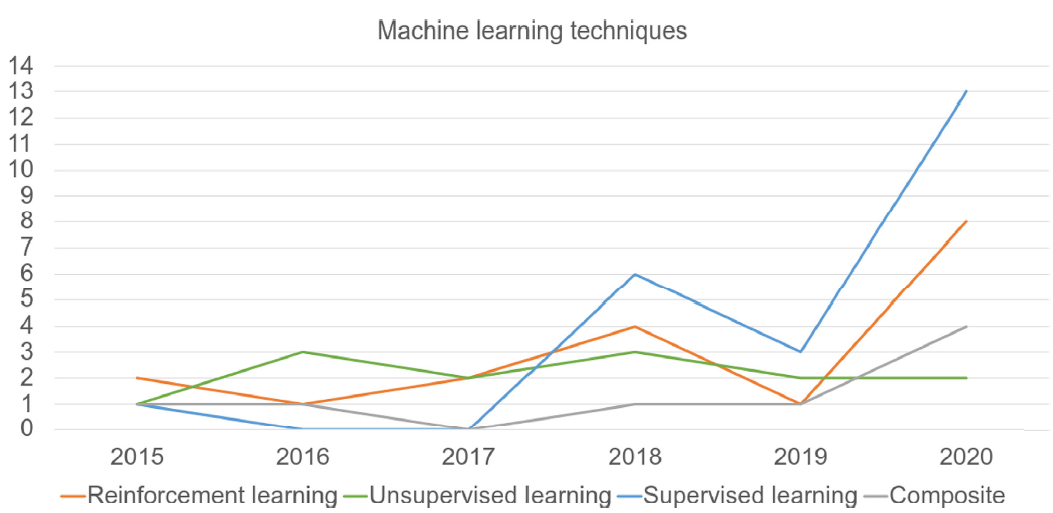
\includegraphics[width=6in]{figs/machinelearning.PNG}}
\caption{Number of articles relevant to the HRC review from each machine learning technique throughout the years\cite{Semeraro2023}}
\label{machinelearning}
\end{figure}
\fi

\subsubsection{Supervised Learning}

In Supervised Learning, the models are trained using a dataset of labeled data. According to \textcite{Sarker2021}, these models must generalize the knowledge from the dataset's input-output pairs to correctly deal with a new input they have never seen before. The models from this group are further divided into classification, where the new input is assigned a discrete output class, and Regression, where it is returned a real number from the continuous output space. Currently, \acs{rnn}s and \acs{cnn}s are two of the most common classification approaches.

A \acf{rnn} is a type of neural network where the output of each time step is fed back into the input at the next time step, allowing the network to remember and incorporate information from previous time steps into its processing of current and future data. This characteristic makes \acp{rnn} particularly well-suited to processing sequential data, such as text, speech, or time series data which require context or temporal dependencies. In particular, according to \cite{lstm_advantages}, \acf{lstm} is an \acs{rnn} with a more complex architecture that gives it an improved ability to backpropagate the error, making it better to train a model that classifies sequences with several time steps.

A \acf{cnn} is a type of neural network made up of several convolutional layers which apply a sliding filter over the input reducing its dimension and obtaining its features. Typically, these layers are followed by one or more fully connected layers that perform the prediction using the mentioned features. This architecture makes \acp{cnn} an excellent choice to deal with data in a matrix structure such as an image because this input is too massive for manual feature engineering.

In Supervised Learning, transfer learning is a technique that makes use of a trained external model. Depending on the goal of its use, these models can be entirely or partially used; optionally, they can also be trained partially or fully. A common use case for this technique is when a small dataset of images is used to obtain a classifier, and a standard model cannot generalize from that reduced amount of data. In this case, a model such as VGG-16 and ResNet-50 can be used partially to extract the features with one or more fully connected layers in the end, to perform the desired classification from those features.

\subsubsection{Unsupervised Learning}

%You say too little on this. Could you say more, or perhaps complement with an example?

In Unsupervised Learning, the datasets involved have no labels. According to \textcite{Sarker2021}, these algorithms aim to find patterns and structure in the data. This makes them valuable in tasks such as clustering based on common characteristics, density estimation, identifying anomalies and outliers, dimensionality reduction, feature learning and finding association rules.

Clustering is a technique used to create groups of points representing instances of the dataset to discover relevant trends or patterns. K-means clustering is one of the most common and simple clustering algorithms. It starts by creating $k$ random centroids and assigns each instance of the data to the closest centroid by squared distance. This process can be repeated to achieve better results. This algorithm works well when the points from different sets are considerably separated from each other.

Dimensionality reduction is a technique that aims to reduce the number of features by selecting a subset of the original ones using algorithms such as Chi-squared test or extracting new features from the originals using algorithms such as Principal Component Analysis (PCA).

%\textcolor{red}{Association Rule Learning is another possible example}

\subsubsection{\acf{rl}}

\acl{rl} is different from the previous approaches because it does not need a dataset. According to \textcite{Alom2019}, the agent learns how to act in an unknown environment by interacting with it. After the agent's action, the environment returns an observation and a certain reward to the agent depending on the quality of the action. The agent uses the reward to update its internal model named policy improving its future performance and the cycle repeats, as shown in Fig.~\ref{rl_diagram}. This type of learning by trial and error has a certain resemblance to how humans gain knowledge, and it is useful when there is a need for an agent to make decisions in an environment that has considerable complexity, such as controlling a robot or playing a game.

\begin{figure}[!ht]
\centering
%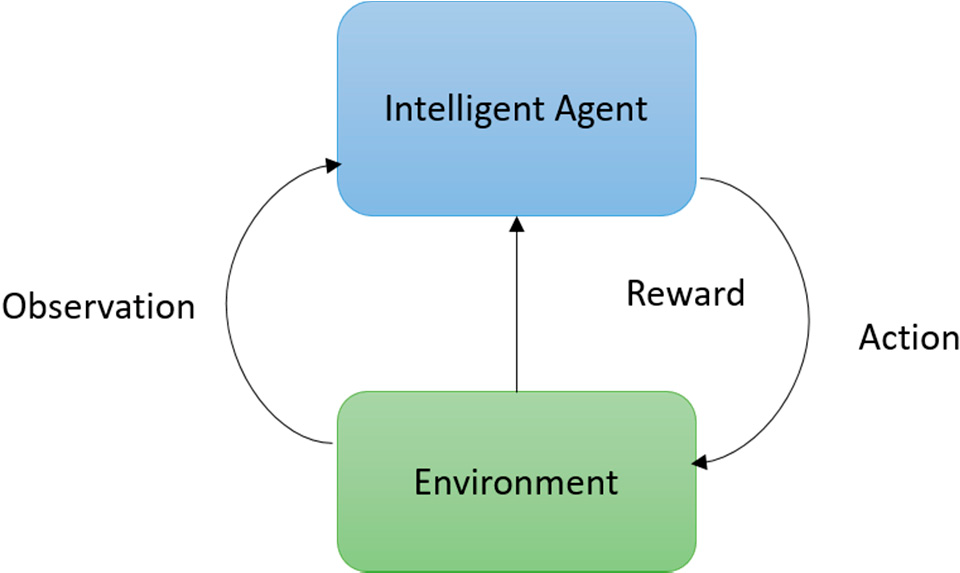
\includegraphics[width=7cm]{figs/rl_diagram.png}
%Alternative in tikz :-) vsantos
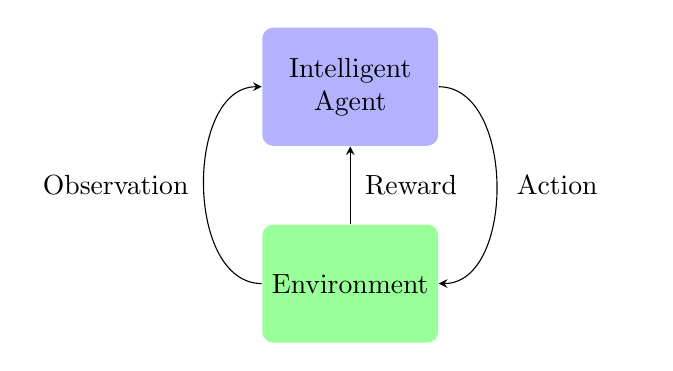
\begin{tikzpicture}[minimum height=1.5cm, text width=2cm, align=center,rounded corners,node distance=2.5cm]
\node [fill=blue!30] (IA) {Intelligent Agent};
\node [fill=green!40,below of=IA] (Env) {Environment};
\draw [->,>=stealth](Env) -- node [midway,right,xshift=-10pt] {Reward} (IA);
\draw [>=stealth] (IA.east) edge[->, in=0,out=0] node [midway,right,xshift=-10pt] {Action} (Env.east);
\draw [>=stealth] (Env.west) edge[->,in=180,out=180] node [midway,left] {Observation} (IA.west);
\end{tikzpicture}
%End of alternative -- vsantos
\caption[Interactions between the Agent and the Environment in \acs{rl}]{Interactions between the Agent and the Environment in \acs{rl} \cite{Alom2019}}
\label{rl_diagram}
\end{figure}

In the workflow of \acl{rl}, the agent must associate an observation to an environment state. This is a simple process in a small discrete environment since there are fewer states. However, if the environment has many variables or it is not discrete then it becomes challenging to associate states with an observation. In these cases, it is necessary to use deep \acl{rl}, which is able to extract the relevant information from the observation and use it to associate the observation with a state.

Given that to train a \acl{rl} model, it is necessary for the agent to interact with the environment thousands of times, this process ends up needing a simulator. According to \textcite{Li2023}, one of the major challenges in \acs{rl} is transferring the knowledge learned in the simulator to a real-life environment. There may be a gap between the real and the simulated environment because the real world has more or less observable variables causing a drop in performance. \textcite{Ahmed2020} also claims that this may be due to an incorrect design of the reward function leading to over-fitting and sub-optimal policies.

\subsection{Collaborative Robotics}
\label{subsection:collaborative_robotics}

\acf{hrc} consists of robots and humans working in the same workspace towards a common goal. Classical industrial robots are usually automated to perform repetitive tasks that require high physical strength. On the other hand, tasks that require cognitive knowledge, flexibility, and precision are better suited for humans, even if they are physically weaker. \acs{hrc} aims to take advantage of both of their strengths and complement each others' weaknesses to increase manufacturing efficiency.

In a \acs{hrc} scenario, robots need to be different from the traditional ones, given that they will work in the same workspace as humans. According to \textcite{Castro2021}, \textquote{Collaborative robots need to be endowed with a set of abilities that enable them to act in close contact with humans, such as sensing, reasoning, and learning. In turn, the human must be placed at the centre of a careful design where safety aspects and intuitive physical interaction need to be addressed as well.}. In \cite{CobotsWW}, it is stated that nowadays, collaborative robots are developed to be compact, easy to install and program, flexible, mobile, consistent and precise. Additionally, they positively impact employees since they are responsible for monotonous and dangerous actions and reduce the production cost for the company.

\subsubsection{Human-Robot Communication}

Humans and robots can communicate through several methods, which can be direct such as using a console or a remote, or indirect, resulting from data captured from sensors. Based on \cite{Castro2021, Mukherjee2022, Semeraro2023,}, the main methods for indirect communication can be seen in the diagram in Fig.~\ref{interaction} and can be described as follows:

\begin{figure}[ht]
\centering
%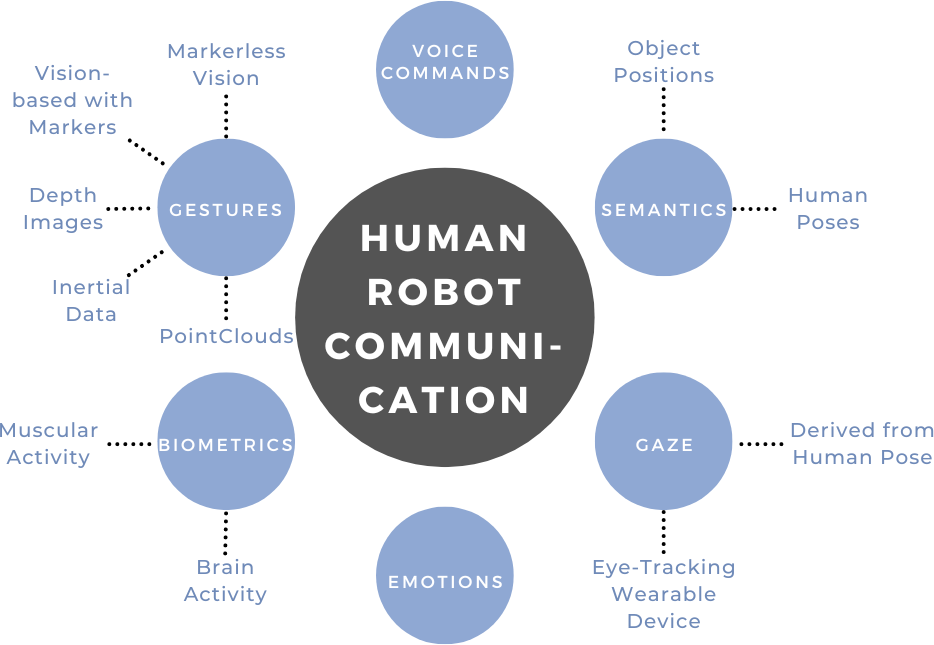
\includegraphics[width=5.5in]{figs/interaction.png}
%% by vsantos, 23 Mar 2023
\definecolor{vColorA}{HTML}{545454}
\definecolor{vColorB}{HTML}{8fa8d3}
\begin{tikzpicture}[scale=0.75,transform shape,
	mindmap,
	grow cyclic,
	every node/.append style={
				concept,
				inner sep=0pt,
				concept color=vColorB,
    font=\sffamily,
				}, %this is appended to all local props!
	concept color=vColorB,
	text=white,
%	font=\sffamily\bfseries\Large,
	level 1/.append style={
%							level distance=5cm,
%							sibling angle=60,
	%						font=\sffamily,
%							concept color=vColorB,
							},
	level 2/.append style={
%							level distance=2.75cm,
							sibling angle=45,
%							font=\small \sffamily,
							text=black,
%							concept color=white,
						  },
]

\node[] (HRC) at (0,0){\large\bfseries HUMAN ROBOT COMMUNICATION}
	[counterclockwise from = -30]
child[]
{
	node[](Gaze){GAZE}
	[clockwise from = 0]
	child{node[](dhp){Derived from human pose}}
	child{node[](eye) {Eye-tracking Wearable Device}}
}
child[]
{
	node [] (Semantics) {SEMANTICS}
	[counterclockwise from = 0]
	child{node[](hp){Human Poses}}
	child{node[](op) {Object Positions}}
}
child[]
{
	node [] (VoiceCommands) {VOICE COMMANDS}
}
child[]
{
	node []  (Gestures) {GESTURES}
		[counterclockwise from = 60] %[grow=180]
		child{node[](mv){Markerless Vision}}
		child{node[](vbm) {Vision based with Markers}}
		child{node[](di) {Depth Images}}
		child{node[](id) {Inertial Data}}	
		child{node[](pc) {Point clouds}}	
}
child[]
{
	node [] (Biometrics) {BIO-METRICS}
		[counterclockwise from = 180]
		child{node[](ma){Muscular Activity}}
		child{node[](ba) {Brain Activity}}	
}
child[]
{
	node [] (Emotions) {EMOTIONS}
}
;

\end{tikzpicture} %an optional representation :-) %vs

\caption{Data sources common in \acl{hrc}}
\label{interaction}
\end{figure}

\begin{itemize}
\item \textbf{Gestures}: these are one of the main ways humans communicate, whether through simple movements or formal sign language. In the literature about \acs{hrc}, gestures can also commonly be found since they have the advantage of resisting ambient noise. Usually, gestures are captured with vision-based methods with either an RGB or RGB-D camera, so there is no need for unnatural movements. With vision, it is possible to include markers, but these may lead to occlusions and hinder the worker's movements. Consequently, there is also work in the literature that uses markerless vision to allow more unrestricted movements. Another way to capture the movements of the human worker would be to use wearable inertial sensors, which contain accelerometers and gyroscopes, but, once again, wearables can hinder the worker's movements. Finally, capturing point clouds using a LIDAR presents another possibility of capturing gestures without restricting the worker's motion.

% Do you mean spoken language by means of sound or written or typed text, or can it be more than this?

\item \textbf{Voice Commands}: Talking is the most intuitive way for humans to communicate with each other. The advances in voice recognition and natural language processing make this a possible communication solution with robots. However, despite being intuitive, simple, effective, and even robust against lighting variations, when it comes to an industrial setting that contains significant sound noise, it becomes less valuable than the alternatives.

\item \textbf{Semantics}: semantic information about the objects can also help the global workflow. For example, suppose the robot is trained to recognize certain features in objects related to how it can pick them up. In this case, the robot can pick up a new object it has never seen before if it has a similar structure. Human actions can also be represented semantically by obtaining the poses of the human as a specific set of limbs, even if only partially. During action recognition, this can be used to know which objects the worker can interact with. Having semantic information about the pose of the human body also helps in the path-planning phase of the robot since it can use this information to avoid the worker and prevent collisions.

\item \textbf{Gaze}: this can be used to determine where the user's attention resides, giving a considerable amount of information that can trigger some action. There are two options to obtain the user's gaze. Wearable sensors can provide better results but are expensive and intrusive. On the other hand, algorithms that detect head pose and assume the gaze from it can also be used, which is a cheaper and non-intrusive solution.

\item \textbf{Emotions}: although this is a relatively new idea, some applications analyze the user's emotions from his facial expressions to have even more information in the algorithms.

\item \textbf{Biometrics}: \acf{emg} sensors can measure electrical signals generated by muscle contractions, while electroencephalography (EEG) signals are commonly used in brain-computer interfaces (BCIs). %\textcolor{blue}{And why not heart beat, breath, ...?}

\end{itemize}

\subsubsection{Safety}

Safety is one of the most critical topics in collaborative robotics and the first step toward establishing a collaborative environment. According to \cite{CobotsWW}, collaborative robots are able to safely work with people because they have sensitive sensors that can detect the human interrupting them, causing them to stop their actions, while traditional robots would potentially injure the worker. However, given that there are tasks that require the robot to move very close to the worker, some norms were implemented: ISO 10218-1 and 10218-2. From these two standards, \textcite{Castro2021} and \textcite{Villani2018} describe the four criteria from which at least one must be met as:
\begin{enumerate}
  \item \textbf{Safety-rated monitored stop}: when a human enters the cobot's workspace, it completely stops;
  \item \textbf{Hand guiding}: when an operator manually moves the cobot, it is compliant;
  \item \textbf{Speed and separation monitoring}: as the human moves closer to the cobot, it becomes gradually slower;
  \item \textbf{Power and force limiting}: the cobot has its operation restricted in terms of force and torque.
\end{enumerate}

\begin{figure}[ht]
\centerline{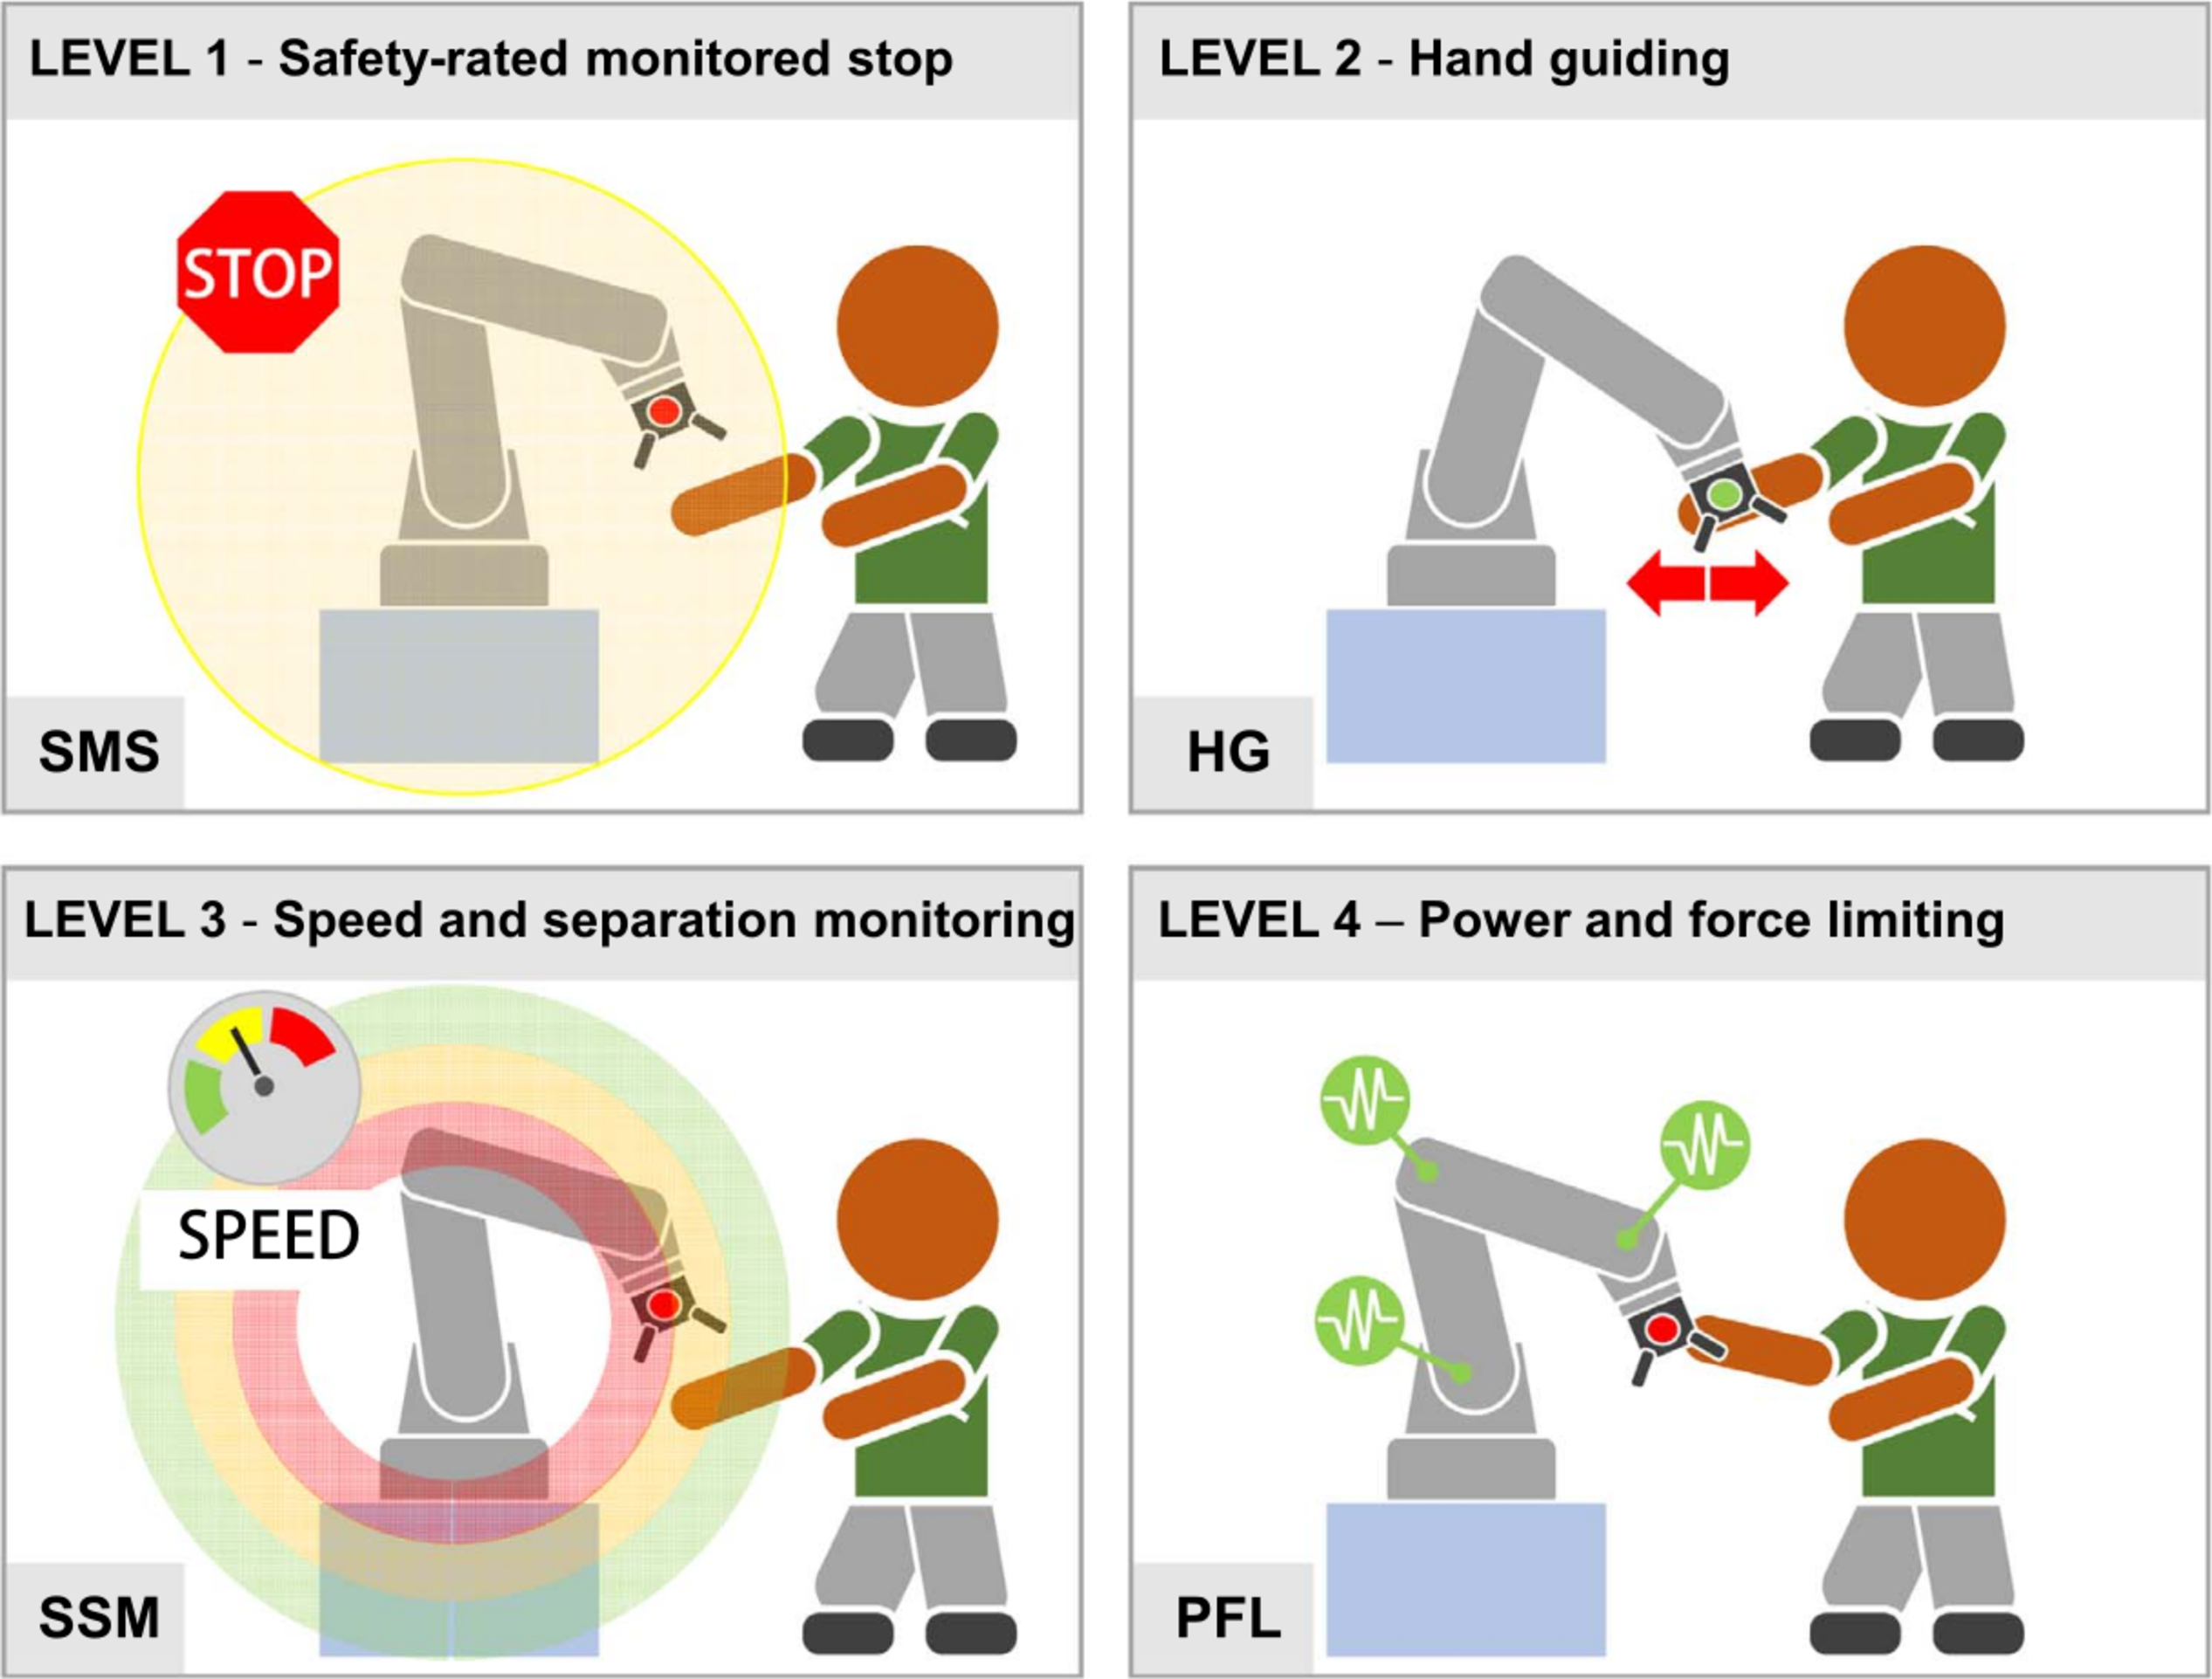
\includegraphics[width=5in]{figs/iso.png}}
\caption[The four collaborative operative modes identified by robot safety standards ISO modes 10218-1/2]{The four collaborative operative modes identified by robot safety standards ISO modes 10218-1/2 \cite{Villani2018}}
\label{isonorms}
\end{figure}

\section{Data Sources and Sensors}

The first step to anticipating the following action is to know which sensors should be used. Previously, several forms of communication between humans and robots were described. Still, these work in a more active way, and not all of them can be applied to action anticipation, where the user should not need to do anything for the robot to act. Essentially, there is a need to capture the human's body language or, in other words, his involuntary pose, gestures and gaze, which became some of the most commonly used data to perform action anticipation.

Regarding the sensors used to capture the raw data, most literature suggests using an RGB camera. However, the captured images may be used in the following different ways:

\begin{itemize}
\item directly used as input to models which can extract features from the images;

\item used as input to frameworks that receive an image, process it, and return the key points, such as the skeleton joints of the person in the image; these key points can also then be used to assume the gaze of the human in the image such as in \textcite{Canuto2021} where the authors used OpenPose (explored in detail in Section \ref{section:keypointdetection}) to obtain not only the skeleton joints but also the worker's gaze;

\item used to process the optical flow\cite{Gammulle2019, Wu2021, Rodriguez2019, Furnari2021};

\item if the human was wearing markers, the image can be used to obtain the positions of the markers obtaining gestures from the sequence of those positions \cite{Maeda2016};
\end{itemize}

Besides RBG cameras, some works, such as the one described in \textcite{Moutinho2023}, indicate the use of an RGB-D camera to capture both the color and the depth images, which contain the gestures and pose of the worker. Other than cameras, in \textcite{Tortora2019} \acs{imu} and \acs{emg} data was used as input to capture the gestures and anticipate the worker's action. When it comes to obtaining the worker's gaze, it is possible to do so from the RGB images as mentioned above, but it is also possible to use wearable sensors to capture it, such as in \textcite{Schydlo2018}.

\section{Methods}

% 1 modelo
% 2+ modelo
% modelo+decision making
% modelo+decision making+motion planning

After knowing which data is usually captured and provided to an algorithm, this section explores possible algorithmic solutions present in previous work starting by those that are only about predicting the action of the human worker and then those that go a step further and reference how to go from a prediction to the action that the robot must execute as a response.

\subsubsection{Predictive Modeling Techniques}

Predicting the next action of the worker can be represented as a classification problem since it is possible to use a sequence of images that must be classified as a particular future action class. Using Fig.~\ref{superviseddiagram} as an example, the high-five action should be predicted before the frames that contain it are captured. The previous work with this kind of algorithm mainly includes \acp{cnn} and \acp{rnn}, with the latter being the most common.

\begin{figure}[!ht]
\centerline{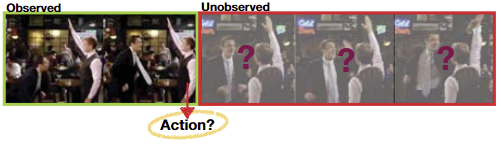
\includegraphics[width=6in]{figs/superviseddiagram.PNG}}
\caption[Action Anticipation using Supervised Learning diagram]{Action Anticipation using Supervised Learning diagram\cite{Gammulle2019}}
\label{superviseddiagram}
\end{figure}

% LSTM only examples
In \textcite{Furnari2021}, the authors aimed to predict the subsequent actions that someone wearing a camera would perform and the objects he would interact with. They used three datasets containing RBG frames from which they derived the optical flow and the objects in the environment. This data is then passed on to a Rolling-Unrolling \acs{lstm}. The Rolling \acs{lstm} (R-\acs{lstm}) is a network that continuously encodes the received observations and keeps an updated summary of the past. When it is time to make predictions about future actions, the Unrolling \acs{lstm} (U-\acs{lstm}) is used with its hidden and cell states equal to the current ones of the R-\acs{lstm}.

In \textcite{Schydlo2018}, the authors used an encoder-decoder recurrent neural network topology to predict human actions and intent where the encoder and the decoder are both \acs{lstm} cells. At each step, the decoder returns a discrete distribution of the possible actions making this algorithm able to consider multiple action sequences, which are then subject to a pruning method that reduces them to obtain the right action finally. In their work, these algorithms were tested in two different datasets, one containing RGB images with optical markers and gaze information from wearable sensors and another with RGB-D images.

% ResNet-34 + LSTM
In \textcite{Moutinho2023}, the authors aimed to increase the natural collaboration between the robot and the human in an assembly station by interpreting implicit communication cues. The data related to the environment was captured using an RGB-D camera. This data was then passed on to a ResNet-34, a pre-trained neural network that extracted the features from the images. These features are used as the input to a \acs{lstm} to perform human action recognition.

% ResNet-50 + LSTM
In \textcite{Gammulle2019}, the authors aimed to predict future frames while at the same time predicting the following action. In their implementation, they used public datasets with videos from which they obtained RGB images and optical flow streams. To consider both data sources, they also used two ResNet-50's, which are pre-trained networks, one to get the input features from the image and another from the optical flow, and 2 \acp{lstm} to take into account both sequences of inputs. Then the two results are merged into a final classification. They also used two Generative Adversarial Networks (GAN) to generate the subsequent frames, but this is different from the focus of the analysis.

%% VGG-16 + TTM
In \textcite{Wang2021}, the authors used video datasets to train a model that would predict a future action from the observed frames. They used three pre-trained neural networks in their work: VGG-16, TS, and ConvNet, to extract features from the images. Then these features were aggregated using a Temporal Transformer module (TTM), and finally, a progressive prediction module (PPM) would anticipate the worker's future action. This article also addresses the issue of specifying what the algorithm should consider as an action. Although most of the literature often implies that the last frames captured by the camera are considered an action, given that those are the frames that contain the last action made by the user, the authors of this article go into greater detail. They tested and evaluated how many frames should be considered as the last action to obtain the best results using a metric from \textcite{Geest2016} named per-frame calibrated average precision (cAP) calculated with \eqref{eq}. In \cite{Wang2021} it is defined with
\begin{equation}
cAP=\frac{\sum_k cPrec(k) * I(k)}{P},
\label{eq}
\end{equation}
\textquote{... where  calibrated  precision $cPrec=\frac{TP}{TP+FP/w}$, $I(k)$ is an indicator function that is equal to 1 if the cut-off frame k is a true positive, $P$ denotes the total number of true positives, and $w$ is the ratio between negative and positive frames. The mean cAP over all classes is reported for final performance.}.

%% CNN
In \textcite{Rodriguez2019}, the authors aimed to predict the following action by first predicting the following motion images. They used datasets containing videos and then processed them to obtain motion images. These motion images become the input of a convolutional autoencoder network that generates the following motion images. These images are then passed to a \acs{cnn} that processes them and makes action predictions for the future. The final action prediction is obtained from the results of the previous network and those of a second \acs{cnn}, which analyzes the original RGB images.

%% architecture with TSN
In \textcite{Wu2021}, the author's goal was to predict the following action someone wearing a camera would perform after some time. Initially, the optical flow was obtained from the captured images, and both were used as input to the model. The model is comprised of a Temporal Segment Networks (TSN), a \acs{cnn}, and a \acs{lstm} to predict the future frame features and then use them to perform the required classification.

\subsubsection{From Prediction to Planning}

After predicting the next action of the worker, the robot must execute some action as a response to complete the anticipation process. This subsubsection contains articles that go beyond the predictive model and have relevant details for the integration of the model in a controller.

In \textcite{Canuto2021}, the authors aimed to predict the following action using a \acs{lstm}, one of the most common \acp{rnn}. In their work, they used a dataset captured with an RGB camera. From these images, they obtained the objects in the environment, the human skeleton joints extracted over time using OpenPose, and the gaze derived from the joints. Then the three data sources were given to the \acs{lstm} as input to perform the desired classification. In this process, the authors use an adaptive threshold on the uncertainty of the recurrent neural network, which makes the model need a certain level of certainty to classify the action as a particular class. This creates a more robust solution since a standard supervised learning algorithm would predict the class with the highest probability even if the model has low certainty about every category.

% Look-up table
In \textcite{Maeda2016}, the authors aimed to reduce the delay in the robot's response by anticipating the human worker and providing a screw or a plate accordingly. They captured the environment using an RGB camera and tracked the hand using optical markers. Then they predicted the following human action using a look-up table containing different orders for assembly actions. With the nearest neighbor algorithm, the actions of the human would be matched with a particular order. The limitation of this method is that all possible sequences need to be on the table because if they are not there, then the robot will match with a different order which may be undesirable. If the robot eventually notices that it did the wrong action, it would then follow a hard-coded contingency trajectory to return to the pre-grasping position. When performing a handover action, the previously captured data is used to generate possible trajectories and this is given to the feedback controller as a reference.

% LSTM + CNN
In \textcite{Zhang2022}, the authors aimed to predict the intention of the human worker to provide him with the required piece. To achieve this, they used an RGB camera to capture the data from the environment. Then the images are given to a convLSTM framework where the \acs{cnn} part is in charge of extracting features from the input images, and these features are then passed on to the \acs{lstm} to predict the intention. This article also tackles the issue of having several possible assembly orders. It solves it by creating a phase at the beginning of the collaboration in which the robot learns the assembly actions and their order from a demonstration. After the prediction of the intention of the worker, the robot proceeds to fetch the required piece. It uses a \acs{cnn} to recognize said piece and \acs{ros} Open Motion Planning Library (OMPL) to handle the trajectory planning jobs. In terms of safety, the authors defined speed limits for the robot and ensured that the robot would avoid the workspace of the human. Then when it needs to move closer to the user, its speed is reduced to guarantee the user's safety.

In \textcite{Huang2016}, the authors' goal is to make the robot use the anticipated actions of the worker to decide its tasks. It monitors the worker's gaze using a wearable device and uses it to predict his intent using SVM. After predicting it, the robot uses an anticipatory motion planner named \textquote{MoveIt!} to plan its motion according to a certain confidence threshold. This means that while it is unsure of what the human wants, the robot starts to move towards the item it thinks he wants but only really moves completely when it surpasses the threshold.

\if{0}
% POMDP
In \textcite{Gorur2018}, the authors aimed to make the human-robot interaction more natural by detecting unexpected conditions where the human will not need the robot's assistance, such as when the human's current intention is unknown or irrelevant to the robot or when even though the human's intent is relevant, that task is done only by the human. They used the algorithm Partially Observable Markov Decision Process (POMDP) to achieve this. The training was done with simulation with the model learning a policy by having a positive reward if the task was accomplished and a negative reward if the robot tried to help the human in a situation where it should not.

\section{\textcolor{red}{\acl{hrc} Safety}}

\textcolor{red}{potentially join this content with the previous subsubsection}

Finally, safety is a topic that must always be mentioned when robots work with humans, especially in \acs{hrc}. Although this topic was also covered in subsection \ref{subsection:collaborative_robotics}, many articles in action anticipation also explore their strategies to ensure the worker's safety.

In \cite{Psarakis2022}, the authors attempted to create a sense of anticipation in humans towards the robot's movements through visual cues of the robot's upcoming action, which is the reverse of what it is being tried to achieve in the other reviewed papers. As with the previous article, they also made it so the robot must reduce its movement speed when close to the robot. Although it was only tested in the Virtual Reality simulation shown in Fig.~\ref{vr}, where the users feel safer, they concluded that the efficiency of the collaboration was increased, and the user had a greater feeling of safety and trust. Furthermore, knowing what the robot will do next also decreases the risk of a collision since the user will avoid the space where the robot is working, increasing safety.

\begin{figure}[!ht]
\centerline{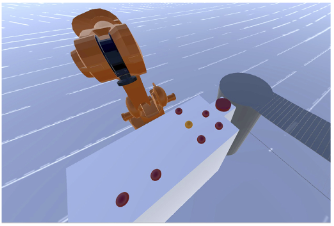
\includegraphics[width=3.5in]{figs/reverse.PNG}}
\caption{VR Simulation of \cite{Psarakis2022}, the orange means the robot will pick that puck next}
\label{vr}
\end{figure}

In \cite{Mukherjee2022}, it is also stated that limiting the power and force of the robot decreases the gravity of the consequences of a possible collision, increasing safety.
\fi